
\chapter{Cadre du projet}
Dans ce premier chapitre, nous entamerons notre rapport en offrant une vue de l’organisme
d’accueil ainsi que le cadre général du projet, dans lequel j’ai effectué mon stage pour le projet
de fin d'études. 
Ce chapitre sera structuré en trois parties
principales. La première partie sera consacrée à la présentation de l'organisme d'accueil, suivie
d'une description globale du projet dans la deuxième partie, et concluant par l'exposé de la
méthodologie de travail.

\section{Présentation de l’organisme d’accueil (Tamtam International)}

Tamtam International est une entreprise de développement et d’intégration de produits et de
solutions web et mobiles. Fondée en 2012 par Monsieur Emmanuel Degrève à Solvay en
Belgique, qui a ouvert son bureau à Marrakech en 2015.
\begin{figure}[htbp]
    \centering
    
\includegraphics[width=0.5\linewidth ]{logos/tamtam-logo.png}
    \caption{ Logo officiel de l'entreprise TamTam International}
    \label{fig:enter-label}

\end{figure}
\vspace{0.5cm} %for just adding space
\subsection{ Fondateur Tamtam International}
Emmanuel Degrève, fondateur et dirigeant de Tamtam International, est la référence en Belgique sur des matières telles que l’impôt des personnes physiques (IPP) et le passage en société. Au-delà des ouvrages qu’il publie chaque année, il est professeur à l’établissement d’enseignement supérieur à Bruxelles (Ephec) et président de Forum For the Future (la fondation qui organise le congrès annuel des professions économiques à Brussels Expo).
% Figure avec l'encadré
\begin{figure}[htbp]
    \centering
    \begin{tcolorbox}[
        enhanced,
        colframe=tamtamblue!50,
        colback=white,
        arc=6mm,
        boxrule=1pt,
        width=\textwidth ]
    \begin{minipage}{0.3\textwidth}
        \centering
        \roundedimage{0.85\textwidth}{image.png}
    \end{minipage}%
    \hfill
    \begin{minipage}{0.65\textwidth}
        \centering
        \textcolor{tamtamblue}{\Large\textbf{DEGREVE Emmanuel}}\\[0.4cm]
        Fondateur de \textbf{Tamtam International}\\[0.4cm]
        Président de la fondation \textbf{Forum For the Future}
    \end{minipage}
    \end{tcolorbox}
    \caption{Fondateur de Tamtam International}
    \label{fig:emmanuel-degreve}
\end{figure}

% \clearpage  % Force a page break or use
\vspace{0.5cm} %for just adding space

\subsection{l'origine de la nomination tamtam}
Il a choisi son nom en s'inspirant symboliquement de l'instrument de percussion \textbf{tam-tam}.
Le tam-tam traditionnel est historiquement utilisé en Afrique et ailleurs comme un moyen de \textbf{communication à distance}, transmettant des messages codés entre villages.
De même, Tamtam International se spécialise dans la \textbf{gestion de communautés} et la facilitation des interactions, reflétant cette idée de \textbf{connecter les personnes} à travers des outils modernes, tout comme le tam-tam reliait les communautés autrefois.
\begin{figure}[htbp]
    \centering
    \begin{minipage}{0.4\linewidth}
        \centering
        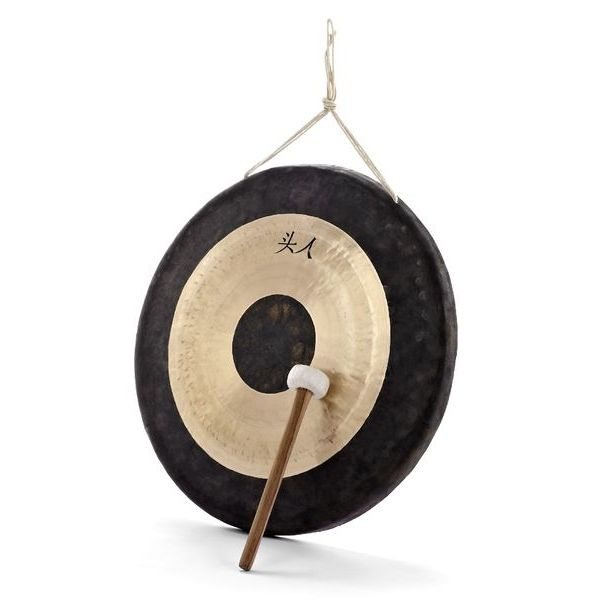
\includegraphics[width=\linewidth]{Chapters/tam-tam.png}
        \caption{Tam-tam}
        \label{fig:image1}
    \end{minipage}
    \hfill
    \begin{minipage}{0.45\linewidth}
        \centering
        
\includegraphics[width=\linewidth]{logos/tamtam.png}
        \caption{logo Tamtam international}
        \label{fig:image2}
    \end{minipage}
\end{figure}

\subsection{Activité de tamtam International}
L'entreprise Tamtam se distingue des autres entreprises sur le marché par sa philosophie ; elle ne
se spécialise pas dans le développement de solutions informatiques pour d'autres clients à la
demande, mais elle se focalise sur le développement d'un écosystème pour la gestion de
communautés et vise à devenir le leader sur le marché.
\subsection{Produits de Tamtam International}
Les produits offerts par Tamtam sont variés et visent à créer un écosystème complet pour la
gestion efficace des communautés. Chaque produit est conçu pour répondre à des besoins
spécifiques, allant de la communication interne à l'engagement des membres. En intégrant ces
solutions, Tamtam permet aux utilisateurs de centraliser les interactions, de faciliter la
coordination et d'améliorer la collaboration au sein de leurs communautés. L'objectif principal est de fournir des outils qui soutiennent la croissance et le dynamisme des groupes, tout en
simplifiant la gestion quotidienne et en renforçant les liens entre les membres.
\begin{figure}[htbp!]

    \hspace{4cm} % Décalage horizontal
    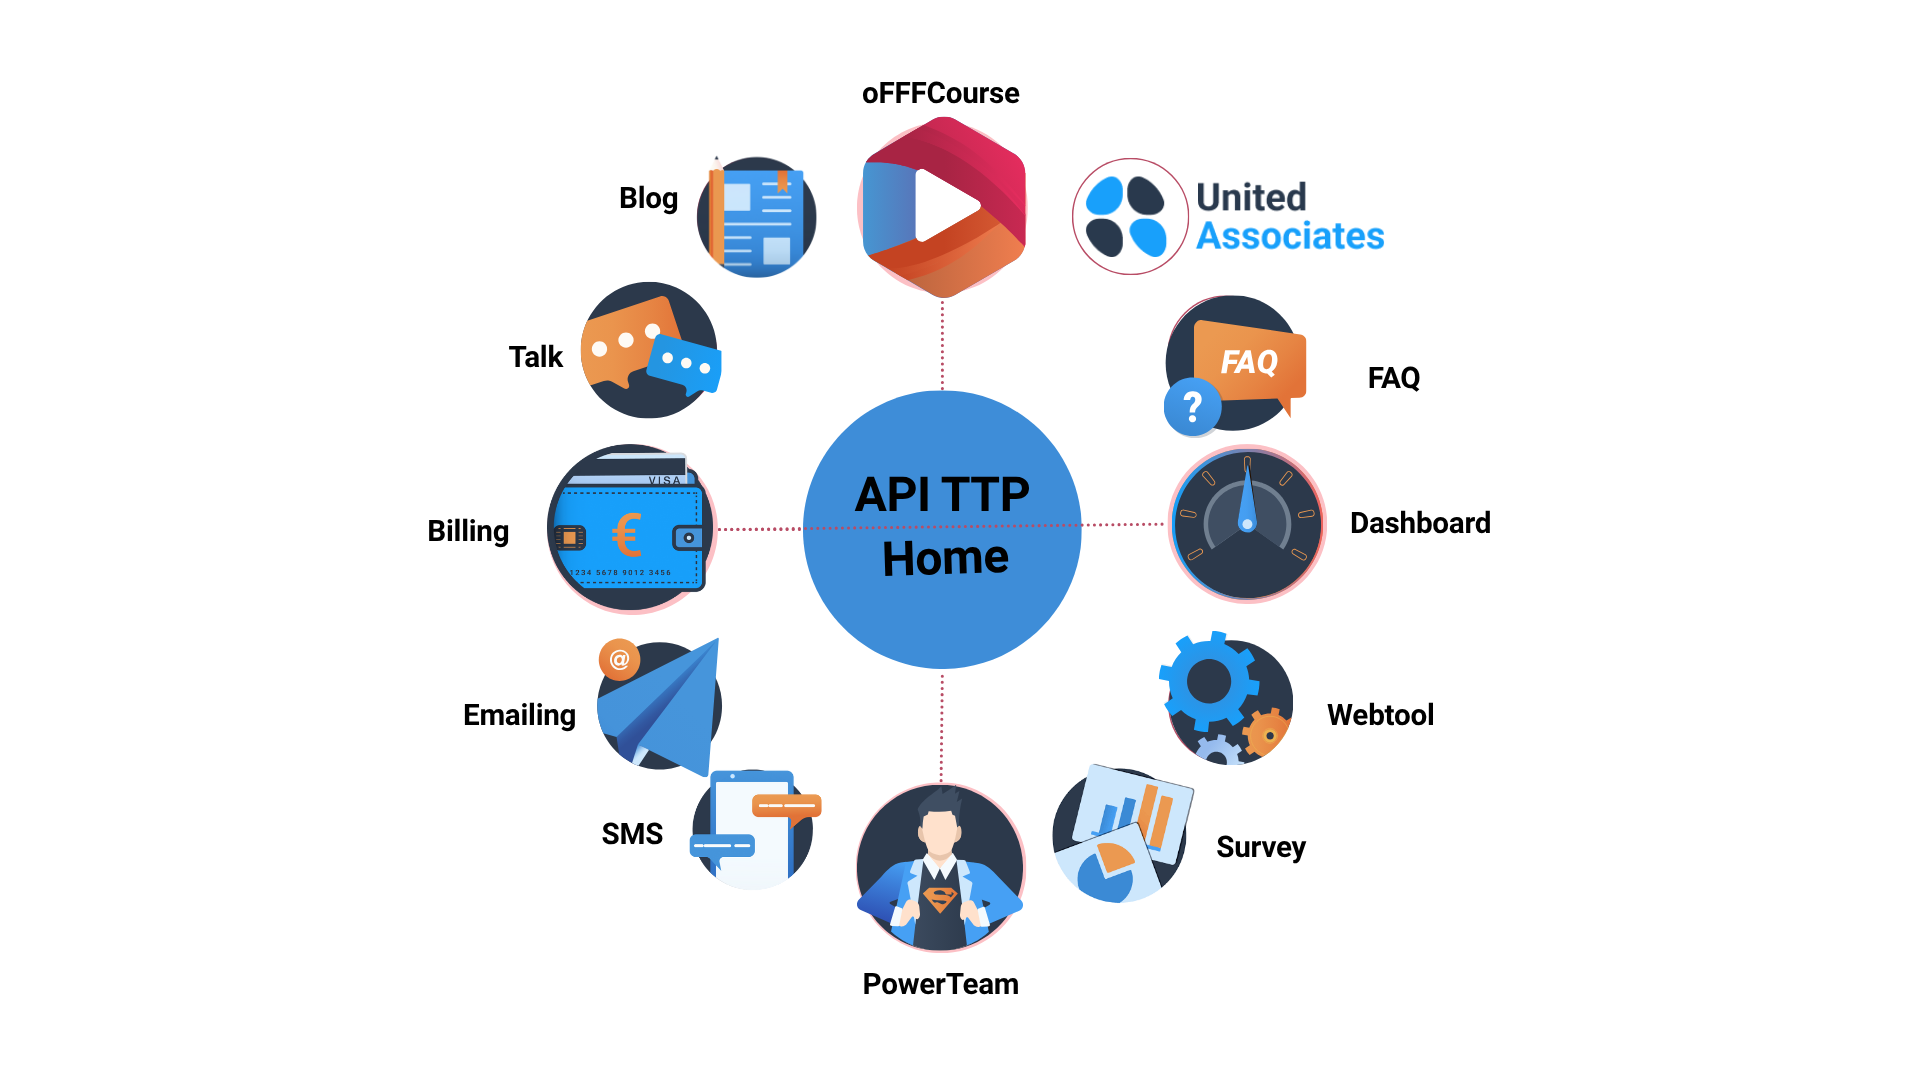
\includegraphics[width=1.55\linewidth, right]{Chapters/produitsTamtam.png}
    \caption{produit tamtam internationel}
    \label{fig:enter-label}
\end{figure}

\textbf{Home} : Cette application centrale représente l’interface d’authentification pour toutes les
applications de Tamtam. Elle gère les différents utilisateurs des organisations en leur offrant la
possibilité d’activer etde configurer les différentes applications disponibles pour chaque profil
utilisateur.

\textbf{Emailling} : Une application permettant à un client d’envoyer des compagnes (des emails) à des
contacts (des utilisateurs stockés dans la base de données dans ttp-users qui ont un email).

\textbf{Blog} : Une application offrant un espace personnel à un utilisateur pour rédiger ses articles,
consulter d’autres articles, ainsi que choisir les organisations qui peuvent le consulter.

\textbf{oFFcourse} : Une application web ayant une partie mobile gérant les événements (conférences,
formations) pour des fiduciaires situés à Belgique. Le visiteur peut consulter le planning, les
orateurs, les places disponibles et s’inscrire à une formation ou réserver une place à une
conférence en choisissant une formule précise parmi celles proposées, ou bien en proposant un
événement.

\textbf{Talk} : est une application interne pour le moment, elle prend automatiquement les clients et
collègues de la personne connectée à Home. Les utilisateurs peuvent chatter, passer des appels
audio et vidéo et envoyer des documents.

\textbf{Billing} : est un moteur de routage permettant le transfert et l’acheminement des
documents électroniques vers la bonne destination, tout en prenant en considération le métier et
les besoins des experts comptables. Un document électronique peut être une facture sous format

\textbf{Efff} ou\textbf{PDF}, un bulletin de paie ou un document bancaire de type Coda.
Paiement : Cette application permet aux clients Tamtam d’effectuer le payement des
évènements ainsi que des produits qu’ils désirent obtenir, elle regroupe deux types de payement
en ligne et prend en charge les virements.

\textbf{Survey} : une application web qui permet de fournir une plateforme pour générer des
questionnaires afin d'offrir à tous les fiduciaires belges les moyens nécessaires pour consulter la
satisfaction de ces clients. De plus gérer les données et les réponses par des Dashboard avec
graphiques et statistiques, qui montreront de manière synthétique les résultats de chaque
questionnaire.

\textbf{SMS} : une application permettant à chaque client (organisation, fiduciaire) d'envoyer des sms à
ses clients qui sont stockés dans la base de données Tamtam qui ont un numéro de téléphone.
Afin de leur permettre de connaître par exemple les dates et thèmes des évènements, les
nouveautés, etc. Cette application utilise une api externe qui s'appelle MessageBird.

\textbf{workflow} : une application permet de piloter les résultats par une réconciliation des tâches
effectuées et de déterminer qui et où se produit la valeur ajoutée et de maximiser la charge à
facturer au client en tenant compte des éventuels gains de productivité.

\textbf{E-zine} : une extension de Blog, elle est accessible juste pour des utilisateurs qui ont un compte,
en lui offrant la possibilité de partager des articles dans les réseaux sociaux et intégrer des
articles externes...

\textbf{Efff-viewe}r : une application gérant la validation des factures au format efff. Ce format est né
le 7 juillet 2012, basé sur l’UBL 2.0 il limite considérablement les champs (réduits à 200
potentiels) et consacre une même interprétation de toutes les maisons de softwares. Un langage
commun voit le jour et permet dorénavant à la majorité des logiciels comptables et de gestion
(80 % du marché) d’émettre et de recevoir sous un même format une facture électronique.
PowerTeam: est une application conçue pour la gestion complète des relations entre les clients
et leurs collaborateurs. Elle offre des fonctionnalités pour la gestion des collaborateurs, leurs
budgets ainsi qu'un outil de suivi des prestations afin d'optimiser leur rendement.

\subsection{Clients de Tamtam International}

Les principaux clients de Tamtam International sont les organisations des fiduciaires et expert-comptable en Belgique, les principaux clients sont :


\begin{itemize}
    \item \textbf{\textbf{IEC }: }Institut des Experts-comptables et des Conseils fiscaux – Belgique.
    \item \textbf{\textbf{UP (UnifiedPost) }: }société belge leader dans le secteur des fintechs.
    \item \textbf{\textbf{Deg \& Partners }:} C'est un bureau comptable en pleine croissance, spécialisé dans les professions libérales, les artistes et les ASBL (association sans but lucratif), et expert dans le passage.
    \item \textbf{FFF (Forum For the Futur) }: le congrés Forum for the Futur est le rendez-vous annuel des professions économiques.
    \item \textbf{ITAA (Institute for Tax Advisors \& Accountants) }: Institut des comptables et des conseillers fiscaux, Belgique.
\end{itemize}

\begin{figure}[htbp]
    \centering
    
\includegraphics[width=1\linewidth]{Chapters/image.png}
    \caption{Clients de Tamtam International}
    \label{fig:enter-label}
\end{figure}
\section{Présentation du projet de stage}
Durant mon passage chez Tamtam International, j’ai eu la chance de contribuer à un projet clé reflétant la volonté de l’entreprise de s’adapter aux attentes diversifiées de sa clientèle fiduciaire en Belgique.

\subsection{Contexte général du projet}

Tamtam Pro se positionne comme une plateforme belge innovante, dédiée à l'accompagnement des professionnels fiduciaires à travers le pays. La particularité de cette structure réside dans son approche modulaire, où chaque projet répond à des besoins sectoriels distincts, nécessitant une adaptation permanente de la part des équipes techniques.

Face à l'expansion continue de l'entreprise, plusieurs fonctionnalités stratégiques ont été progressivement implémentées. Parmi ces développements clés, on retrouve notamment des outils avancés de gestion budgétaire et d'optimisation de la capacité productive, spécialement conçus pour les cabinets fiduciaires.

Cette initiative s'inscrit dans la philosophie d'innovation permanente qui caractérise Tamtam International, avec pour vocation d'anticiper les évolutions du marché belge des services financiers. Les solutions développées s'adressent principalement aux entreprises partenaires du réseau Tamtam, particulièrement aux fiduciaires qui exercent une activité à forte intensité cognitive et opérationnelle.

La création de ces outils répondait à un double impératif :
 \begin{enumerate}
     \item Simplifier les processus métiers exigeants.
     \item Optimiser le ratio effort/rendement professionnel.
 \end{enumerate}

Structurellement, Tamtam opère actuellement à travers deux pôles complémentaires :
\begin{itemize}
    \item oFFcourse.be (équipe d'accueil de mon PFE)
    \item UnitedAssociate.be
\end{itemize}

\subsubsection{Objectifs du projet de fin d'études}
Mon intervention s'articule autour de deux axes principaux :
 \begin{enumerate}
     \item L'optimisation des fonctionnalités existantes pour répondre aux nouvelles attentes utilisateurs.
     \item Le développement d'un système LMS dédié au management des compétences, permettant :\begin{itemize}
     \item La définition d'objectifs formatifs trimestriels (en heures-crédits).
   \item Un mécanisme de recommandation intelligente de parcours pédagogiques.
  \item Le suivi granularisé des progressions individuelles.
     \end{itemize}
 \end{enumerate}

\subsection{Problématique}
Aujourd’hui, le marché belge de la formation fiduciaire devient de plus en plus concurrentiel, avec des exigences croissantes en matière de suivi et de personnalisation des apprentissages. Face à cette évolution, Tamtam Pro cherche à renforcer son écosystème en y intégrant une nouvelle interface LMS complète, capable de répondre aux besoins spécifiques des fiduciaires.

La question centrale se pose alors : comment Tamtam Pro peut-il réussir cette transition vers un système plus performant, tout en gardant son avantage concurrentiel ?

D’une part, il s’agit d’automatiser le suivi des obligations de formation continues, un enjeu clé pour les fiduciaires soumis à des réglementations strictes. D’autre part, le système doit personnaliser les parcours d’apprentissage en fonction des profils métiers, permettant ainsi à chaque collaborateur de progresser efficacement.

Enfin, cette solution doit se différencier des plateformes existantes, en offrant une flexibilité accrue et des outils de reporting avancés, adaptés aux réalités opérationnelles des cabinets fiduciaires.

En résumé, le défi consiste à concevoir un LMS qui soit à la fois structuré, personnalisable et intégré harmonieusement dans l’écosystème Tamtam, tout en répondant aux attentes précises des professionnels du secteur.

\subsection{Étude des solutions existantes sur le Marché}
\label{sec:solutions-existantes}

Dans le domaine des \textbf{Learning Management Systems (LMS)} dédiés aux fiduciaires et aux métiers réglementés, plusieurs solutions se démarquent. Cette analyse comparative permet d'identifier les \textbf{forces et faiblesses} des plateformes concurrentes, tout en mettant en lumière les \textbf{opportunités d'innovation} pour Tamtam Pro.

\subsubsection{Plateformes généralistes (LMS polyvalents)}
\begin{itemize}
    \item \textbf{Moodle, LearnDash, TalentLMS}
    \begin{itemize}
        \item[\checkmark] \textbf{Avantages} : flexibilité, personnalisation des parcours, outils de suivi basiques.
        \item[\texttimes] \textbf{Limites} : non adaptés spécifiquement aux besoins des fiduciaires.
    \end{itemize}
\end{itemize}

\subsubsection{Solutions spécialisées pour les fiduciaires}
\begin{itemize}
    \item \textbf{FiscalTalent (payroll \& legal training)}
    \begin{itemize}
        \item[\checkmark] \textbf{Points forts} : contenus préétablis pour les formations fiscales.
        \item[\texttimes] \textbf{Défis} : rigidité dans la gestion des objectifs
    \end{itemize}
    
    \item \textbf{Acerta Academy}
    \begin{itemize}
        \item[\checkmark] \textbf{Atouts} : intégration avec les outils RH
        \item[\texttimes] \textbf{Faiblesses} : interface peu intuitive.
    \end{itemize}
\end{itemize}

\subsubsection{Analyse des lacunes du marché}
Les solutions actuelles présentent \textbf{trois principales limites} :
\begin{enumerate}
    \item Manque d'adaptation aux cycles trimestriels
    \item Absence de mécanismes intelligents de recommandation
    \item Peu de flexibilité dans le suivi des formations hybrides.
\end{enumerate}

\subsubsection{Positionnement de Tamtam Pro}
Pour se différencier, le futur LMS \textbf{« Didier »} devra :
\begin{itemize}
    \item[\textbullet] Combler les lacunes des solutions existantes.
    \item[\textbullet] Offrir une expérience unifiée dans l'écosystème Tamtam.
    \item[\textbullet] Automatiser le suivi avec personnalisation fine.

\end{itemize}

\begin{quote}
\textit{Cette étude confirme l'opportunité stratégique pour Tamtam Pro de développer une solution à la fois spécialisée, intuitive et intégrée, répondant mieux aux attentes des fiduciaires que les alternatives actuelles.}
\end{quote}

\section{Conduite de projet}
La gestion et la planification de projet constituent le pilier central pour mener à bien toute initiative. Une démarche méthodique s'impose pour structurer l'ensemble des activités, depuis l'identification précise des tâches jusqu'à leur séquencement optimal. Ce processus exige notamment d'évaluer avec justesse la durée nécessaire pour chaque action et d'établir une chronologie rigoureuse des phases. Cette approche disciplinée permet non seulement de cadrer efficacement le déroulement des opérations, mais aussi de maîtriser les délais et d'anticiper les éventuels aléas. Dans le cadre de notre projet LMS, cette méthodologie prend tout son sens pour garantir une implémentation fluide et conforme aux attentes.
\subsection{Méthodologie de travail}
Le choix d'une méthodologie adaptée constitue un facteur clé de succès pour tout projet informatique, permettant à l'ensemble des acteurs de collaborer efficacement selon des règles bien définies. Cette sélection stratégique doit répondre précisément aux spécifications du projet tout en garantissant un produit final conforme aux attentes clients. Chez Tamtam International, nous avons opté pour Scrum comme méthodologie de référence, pour plusieurs raisons déterminantes : son efficacité éprouvée dans divers contextes projet, sa capacité à se rapprocher au plus près des besoins clients, sa simplicité de mise en œuvre, et la transparence qu'elle offre sur l'avancement des travaux. Cette approche agile permet non seulement d'optimiser la qualité des livrables, mais aussi de maintenir une visibilité constante sur l'état du projet.
\subsection{Répartition des rôles}

Le cadre Scrum distingue trois types de participants :

\begin{table}[h]
  \centering
  \caption{Cycle de vie Scrum}
  \label{tab:cycle-vie-scrum}
  \begin{tabular}{p{4cm} p{10cm}}
    \toprule
    \textbf{Acteur} & \textbf{Description} \\\\
    \midrule
    Product Owner &
      Il est incarné par Monsieur Emmanuel DEGRÈVE.
      Il apporte l’expertise fonctionnelle et opère les arbitrages indispensables à la priorisation des développements. \\
      \\
    \addlinespace
    Scrum Master &
      Il est incarné par Monsieur Youssef IDBRAIM, membre de l’équipe,
      et sa mission principale est d’optimiser la capacité de production
      de l’équipe en l’accompagnant dans une amélioration continue. \\
      \\
    \addlinespace
    Équipe de développement &
      Elle prend en charge la réalisation du produit (planification,
      conception, codage, tests, documentation) sans spécialisation des
      rôles. La particularité d’une équipe Scrum est d’être « auto-organisée »,
      et donc dépourvue de toute hiérarchie. \\
    \bottomrule
  \end{tabular}
\end{table}

Étant donné que Scrum suit un processus itératif, les unités de temps centrales sont le \textbf{Sprint} et la \textbf{Release}.\\

Dans le cadre du projet \textit{Tamtam}, une nouvelle approche est adoptée cette année avec une Release de 6 semaines, au lieu de 4. Cette Release comprend 4 Sprints :\\
- Deux Sprints principaux de 2 semaines chacun \\
- Deux Sprints appelés \textit{Sprint-Release} d’une semaine chacun, dédiés à la mise en production, à la finalisation de la documentation, et à la prise en compte des retours des parties prenantes.\\

Le contenu de cette Release est fixé lors d’une réunion de planification initiale, garantissant ainsi son périmètre.

\subsection{Workflow
}
Nous explorerons les principes fondamentaux de Scrum, une méthodologie Agile populaire pour
la gestion de projets. Cela inclut une compréhension approfondie des rôles, des événements et
des artefacts de Scrum, ainsi qu'une analyse de son workflow typique, qui guide les équipes à
travers les phases de planification, de développement, de revue et de rétrospective.
\begin{figure}[htbp]
    \centering
    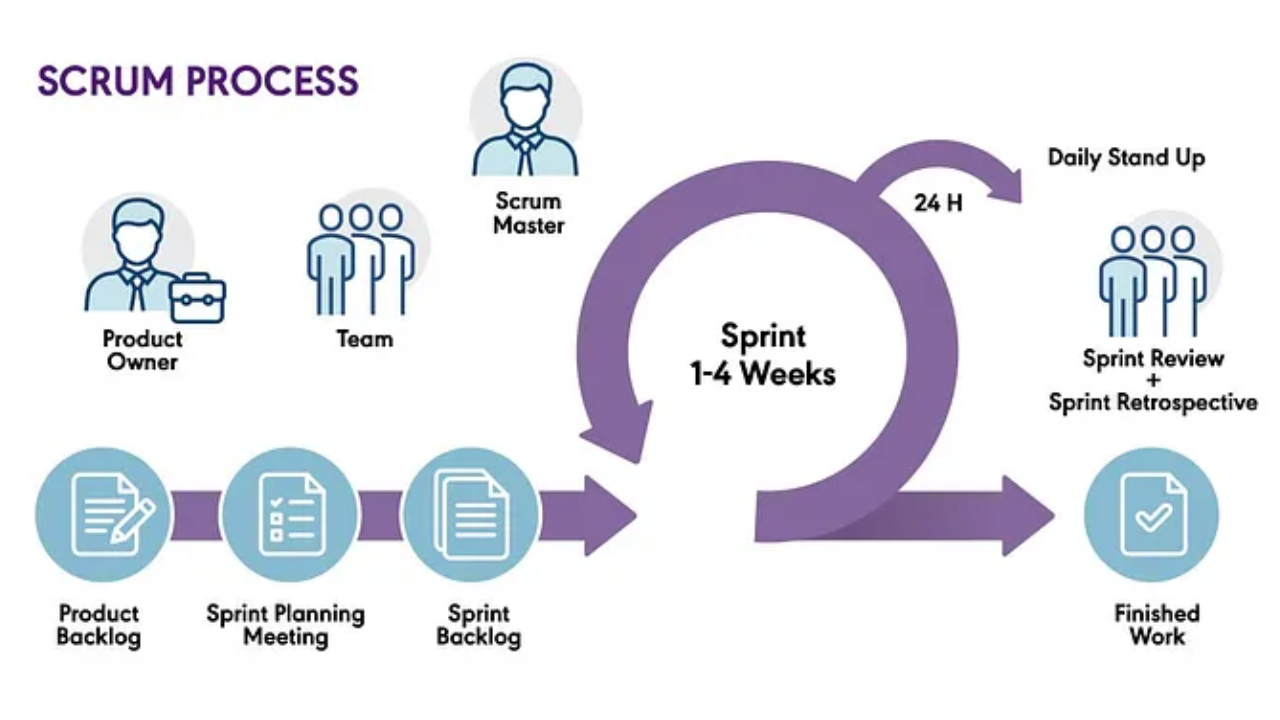
\includegraphics[width=1\linewidth]{Titre de la présentation[1].pdf.png}
    \caption{Cycle de vie SCRUM}
    \label{fig:enter-label}
\end{figure}
\subsubsection{Sprint planning:}
Sprint planning est une étape clé dans la méthodologie agile, particulièrement dans le cadre de
Scrum. Elle vise à définir le travail à accomplir lors du prochain sprint.
Figure 11 Sprint Planning meeting

- L'équipe se réunit pour étudier les exigences fonctionnelles.
- Les fonctionnalités sont divisées en tâches.
- Chaque tâche est attribuée un point par la méthode du planning poker qui représente sa
difficulté.
- Les tâches sont distribuées sur l'ensemble de l'équipe en fonction de l'expertise et des
compétences de chacun.
\subsubsection{Sprint review:}
La Sprint review, dernière étape de chaque sprint Scrum, offre l'opportunité d'examiner
l'incrément de produit. Elle permet à l'équipe de présenter ses réalisations aux parties prenantes,
de recueillir leurs retours et d'ajuster le backlog produit en conséquence. Cette réunion favorise
la transparence et la collaboration, garantissant que le produit évolue de manière alignée sur les
besoins du client tout au long du processus de développement.\\
- L'équipe s'assemble pour présenter une démonstration au PO (Product Owner).\\
- Le PO valide l'état d'avancement et propose des changements.\\
- Le PO spécifie aussi et explique le BR (Business Requirement) à développer pour le
prochain sprint.\\
Durant cette période de stage, nous avions l’habitude d’effectuer deux autres types de réunions :
\subsubsection{Stand up meeting (Daily scrum meeting):}
Chaque jour, nous faisions une petite réunion avec le Scrum master, pour savoir ce qui a été
complété, ce qui est en cours ou planifié, les problèmes et obstacles rencontrés.

\subsubsection{La réunion de rétrospective (Sprint retrospective):}
La rétrospective eut lieu juste après la sprint review, pour discuter le feed-back sur ce qui a été
réalisé, proposer des améliorations du produit, planifier le prochain sprint et assigner les
nouvelles tâches.

\subsection{Gestion des tâches et suivis}
Au sein de notre équipe, Notion joue un rôle central dans la gestion, la collaboration et le suivi
de nos projets. Cet outil polyvalent nous permet de structurer nos tâches, de collaborer de
manière efficace et de maintenir une visibilité claire sur l'avancement de nos projets. Grâce à ses
fonctionnalités flexibles, nous pouvons personnaliser notre espace de travail pour répondre aux
besoins spécifiques de chaque projet, ce qui contribue à une gestion efficace des ressources et à
une coordination harmonieuse des efforts d'équipe.
\begin{figure}[hb!]
    \centering
    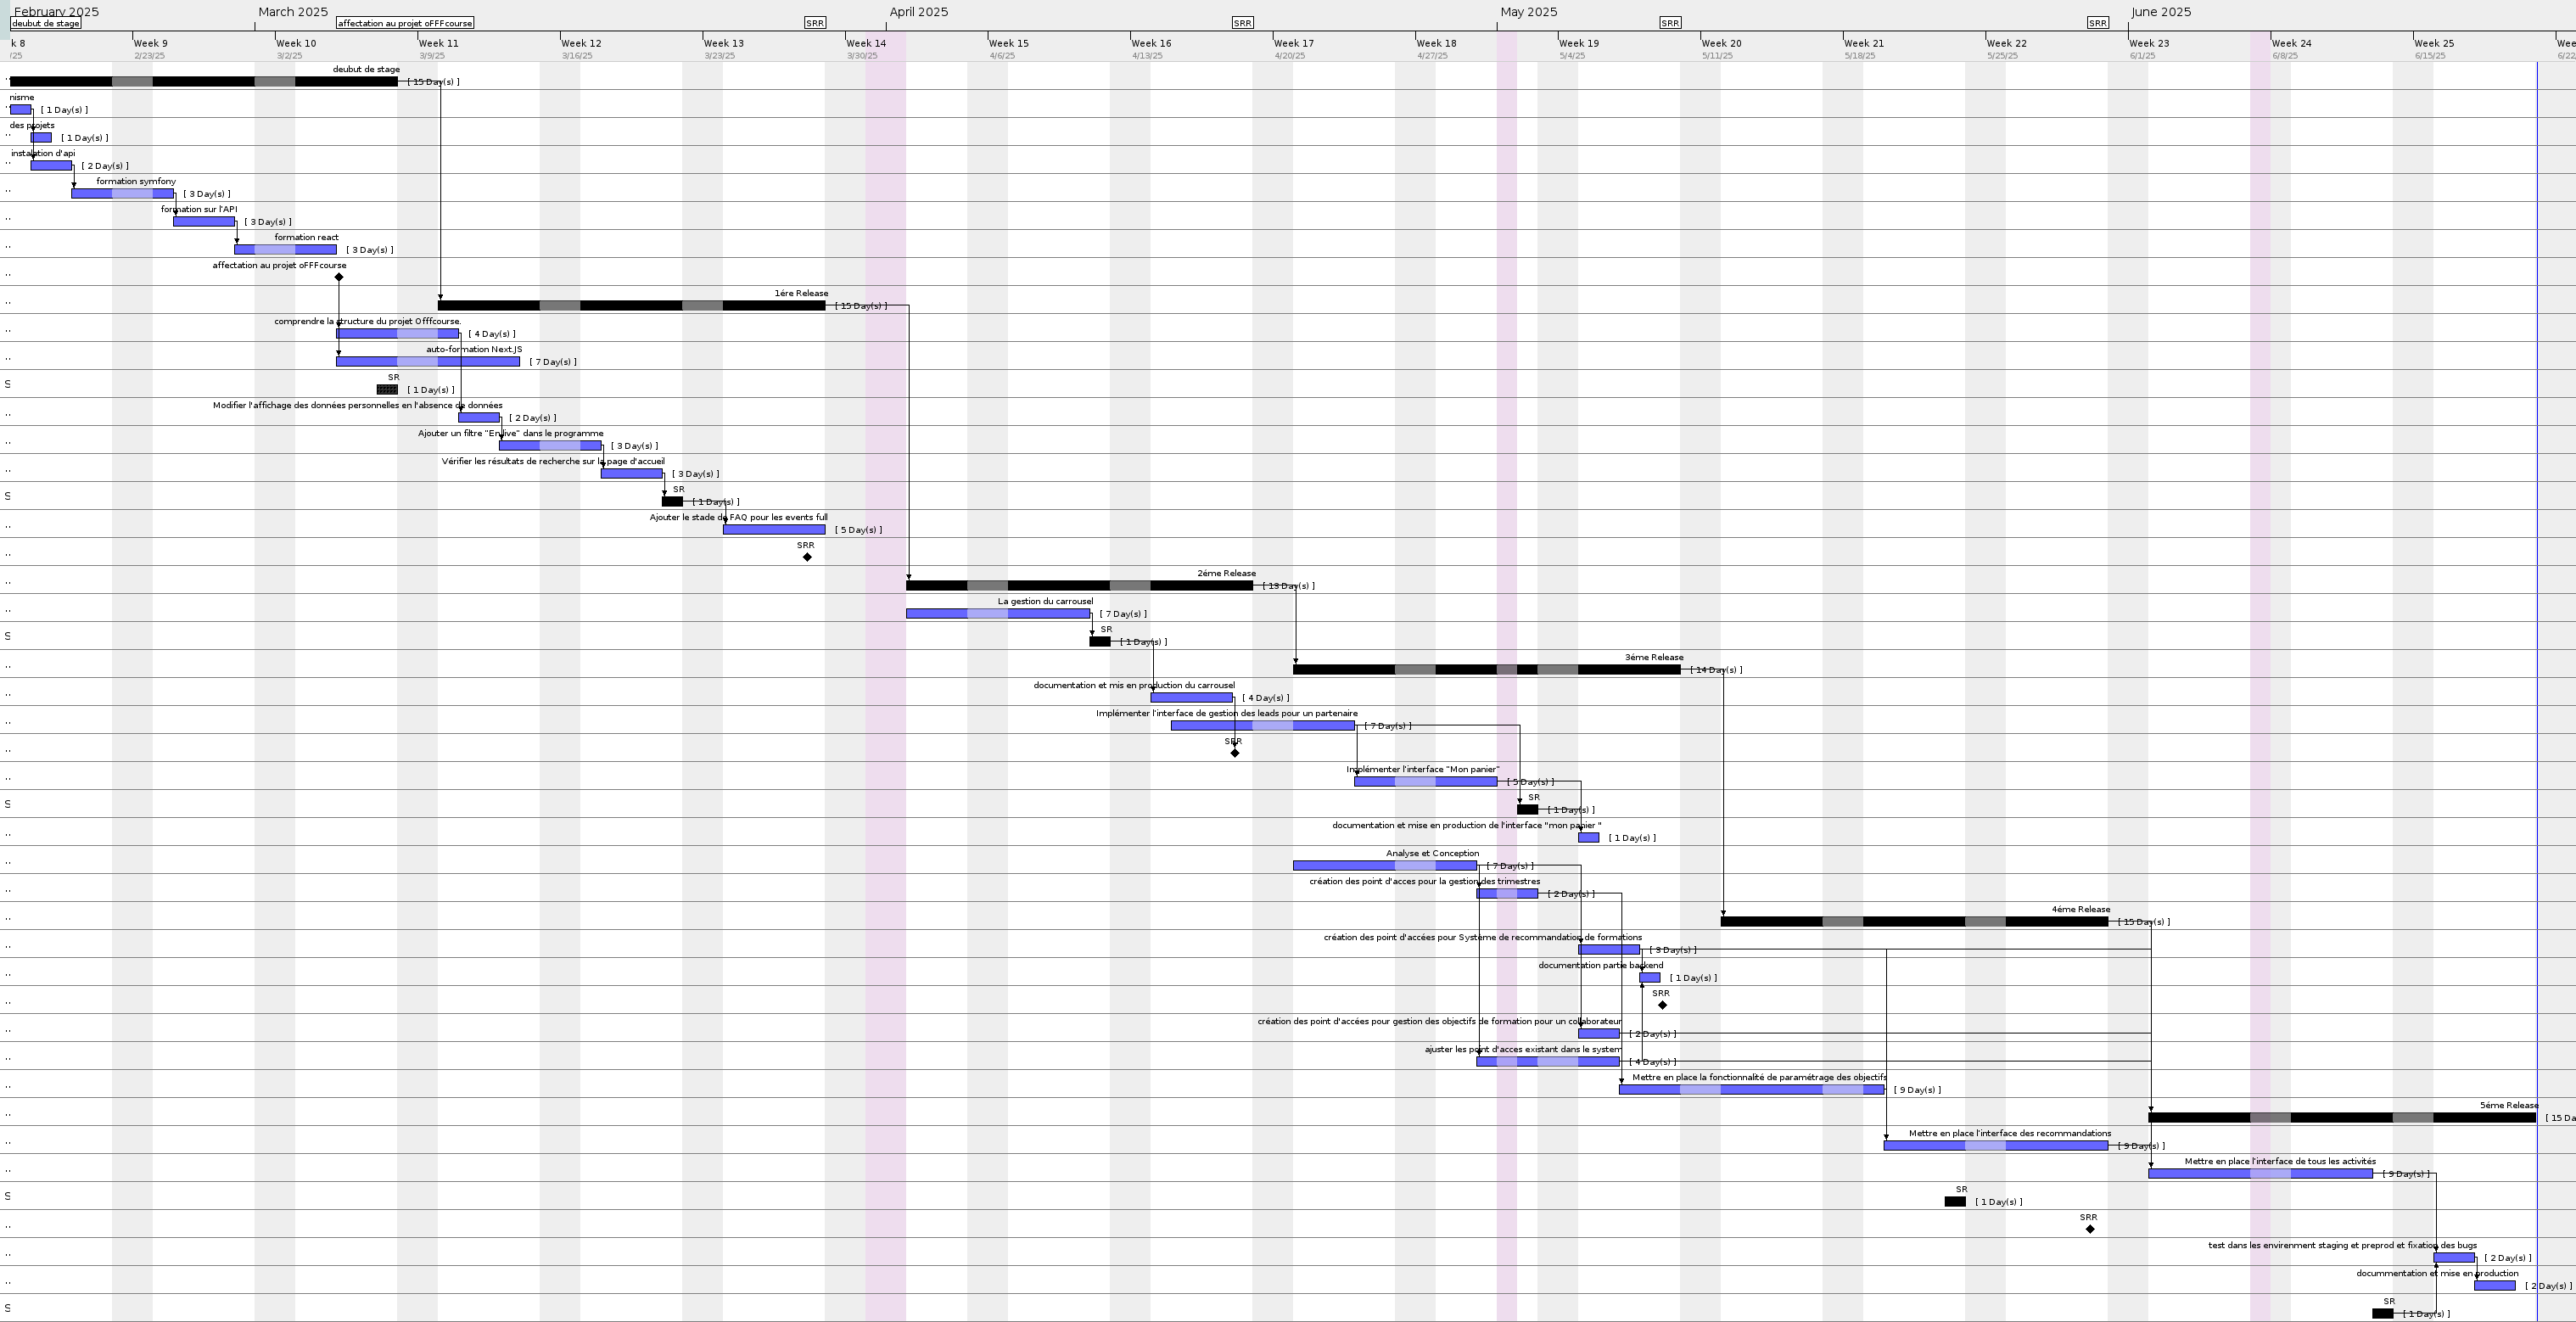
\includegraphics[width=1\linewidth]{pfeProject.gan_page0.png}
    \caption{diagramme de gant }
    \label{fig:enter-label}
\end{figure}
\subsection{Description du diagramme de Gantt}

Ce diagramme de Gantt présente la planification détaillée du projet sur une période de 5 mois (février à juin 2025), intégrant à la fois les tâches liées au développement du système LMS et d'autres activités de l'équipe Tamtam. La structure reflète l'approche Scrum avec des sprints de 2 semaines.

\textbf{Tâches identifiées dans le diagramme :}

\textbf{Sprint 1-2 (Février - début Mars) - Tâches autour oFFFcourse :}
\begin{itemize}
    \item Configuration de l'environnement de développement
    \item Maintenance et amélioration des applications existantes (oFFcourse, Blog, etc.)
    \item Résolution de bugs critiques sur les modules Tamtam
    \item Mise à jour des dépendances techniques
\end{itemize}

\textbf{Sprint 3-4 (Mi-Mars - début Avril) - Début des tâches LMS :}
\begin{itemize}
    \item Analyse des besoins fonctionnels du LMS
    \item Étude des solutions existantes sur le marché
    \item Conception de l'architecture système
    \item Définition des user stories et du backlog produit
    \item Création des maquettes et prototypes UI/UX
\end{itemize}

\textbf{Sprint 5-6 (Avril) - Développement core LMS :}
\begin{itemize}
    \item Implémentation du système d'authentification
    \item Développement du module de gestion des utilisateurs
    \item Création de la base de données des formations
    \item Développement de l'interface d'administration
\end{itemize}

\textbf{Sprint 7-8 (Mai) - Fonctionnalités avancées LMS :}
\begin{itemize}
    \item Implémentation du système de recommandations
    \item Développement du module de suivi des objectifs trimestriels
    \item Création des tableaux de bord et reporting
    \item Intégration avec l'écosystème Tamtam existant
\end{itemize}

\textbf{Sprint 9-10 (Juin) - Finalisation et déploiement :}
\begin{itemize}
    \item Tests d'intégration et de performance
    \item Documentation technique et utilisateur
    \item Formation des utilisateurs finaux
    \item Déploiement en production et mise en ligne
\end{itemize}

Cette planification montre clairement que le développement du LMS représente environ 70\% du temps total du projet, les 30\% restants étant consacrés aux formations et aux activités de maintenance et d'amélioration de l'écosystème Tamtam existant.

\section{Conclusion}

Ce premier chapitre a permis d'établir les fondements solides de notre projet de fin d'études au sein de Tamtam International. L'exploration approfondie de l'organisme d'accueil révèle une entreprise innovante, positionnée comme acteur de référence dans l'écosystème numérique des fiduciaires belges.

La présentation de Tamtam International met en évidence sa philosophie unique : plutôt que de développer des solutions sur mesure pour des tiers, l'entreprise se concentre sur la création d'un écosystème intégré de produits, visant l'excellence dans la gestion de communautés professionnelles. Cette approche stratégique, incarnée par la vision de son fondateur Emmanuel Degrève, positionne Tamtam comme un partenaire technologique de confiance pour les professionnels du secteur fiduciaire.

L'analyse du contexte projet révèle une opportunité stratégique majeure : le développement d'un système LMS spécialisé pour répondre aux besoins croissants de formation continue des fiduciaires. L'étude comparative des solutions existantes confirme l'existence d'un gap technologique que le projet « Didier » ambitionne de combler, en proposant une approche à la fois personnalisée, intuitive et parfaitement intégrée à l'écosystème Tamtam.

La méthodologie Scrum adoptée, avec sa structure de sprints et de releases adaptée aux spécificités du projet, garantit une approche itérative et collaborative. La planification détaillée, matérialisée par le diagramme de Gantt, démontre la faisabilité technique du projet dans les délais impartis, tout en préservant la qualité des livrables.

Fort de ces bases solides, nous sommes désormais en mesure d'aborder les phases techniques du projet avec confiance. Le chapitre suivant se concentrera sur l'analyse approfondie des besoins fonctionnels et non-fonctionnels, préalable indispensable à la conception d'une solution technologique performante et adaptée aux attentes des utilisateurs finaux.